\documentclass[12pt,fleqn]{article}\usepackage{../../common}
\begin{document}
Sonlu Öğeler Metotu (Finite Elements Method -FEM-) - 1

Galerkin, Ağırlıklı Artıklar Metotu (Weighted Residual Method)

WRS diferansiyel denklemleri yaklaşık (approximate) olarak çözebilen bir
metottur, bunu tüm yaklaşık fonksiyonun tanım kümesi üzerinden ağırlıklı hata
artıklarını sıfıra eşitleyerek yapar. Bununla ne demek istediğimizi birazdan
yakından göreceğiz [1, Ders 3].

Örnek olarak [2]'de öğrendiğimiz Euler-Bernoulli kirişlerini tanımlayan denklemi
hatırlarsak,

$$
E I \frac{\ud^4 y}{\ud X_1^4} = q
\mlabel{1}
$$

Biraz düzenleme sonrası

$$
E I \frac{\ud^4 y}{\ud X_1^4} - q = 0
$$

elde ederim. Amacım öyle bir yaklaşık $y$, ya da $y_{approx}$ diyelim, bulmak ki
üstteki denklemi çözebileyim. Bunu $y$ yerine onu yaklaşık temsil edebilen bir
diğer fonksiyonu geçirerek yapabilirim. Bir polinom bu işi görebilir; Pek çok
diğer yöntemin kullandığı tipik bir polinom vardır,

$$
y_{approx} = a_0 + a_1 X_1 + a_2 X_2^2 
$$

diye gider, aslında daha genel olarak olan her terimde ``bir katsayı çarpı
$X_1$'in bir tür fonksiyonu'' gibi bir toplam kullanmak daha iyi olabilir,
bu formda,

$$
y_{approx} = a_0 \phi_0(X_1) + a_1 \phi_1(X_1) + a_2 \phi_2(X_2) 
$$

Daha kısa olarak

$$
y_{approx} = \sum_{i=0}^{n} a_i \phi_i(X) 
$$

Dikkat $\phi_i(X)$ içinde $X$ var bu $X = X_1,X_2,..,X_n$ anlamında, cebirsel
olarak her $\phi$ fonksiyonuna $X$ geçildiğini düşünebiliriz ama her $\phi_i$
tüm $X$ öğelerini kullanmayabilir; üstteki polinom örneğinde mesela $\phi_1$
fonksiyonu sadece $X_1$'i kullanarak bir hesap yapar, diğerleri diğer şekillerde.

Not, $y_{approx}$ gerekli (essential) sınır şartlarını yerine getirmelidir.

Metotun dayandığı ana prensip şudur; eğer çözmeye uğraştığım (1)'deki gibi bir
problemde eğer $y$ yerine $y_{approx}$ kullanırsam

$$
\frac{\ud^4 y}{\ud X_1^4} - q = 0 \qquad
\frac{\ud^4 y_{approx}}{\ud X_1^4} - q \ne 0
$$

tabii ki sıfır olmayan bir sonuç alırdım. Ama $y_{approx}$ eğer $y$'ye oldukca
yakınsa sıfır olmasa bile sıfıra yakın bir sonuç alabilirdim.. belki?

Bu yakınlığı bir artık $R$ ile ölçebiliriz,

$$
R = \frac{\ud^4 y_{approx}}{\ud X_1^4} - q 
$$

Üstteki formül içinde bilinmeyen $a_i$ değerleri var hatırlarsak. O zaman, eğer
``iyi'' $a_i$ değerleri seçebilirsem teorik olarak $y_{approx}$ değeri $y$
değerine yaklaşacaktır, ve dolaylı olarak bu $R$'yi minimize eder. Demek ki
$R$'yi minimize edebilen bir yaklaşım aynı zamanda $y$'yi yaklaşık olarak
çözebilen bir yaklaşım olacaktır. 

Daha detaylı olarak ifade etmek gerekirse $D$ tanım alanı üzerinde ifade edilen
ağırlıklı artık hataların toplamını sıfıra eşitleyerek bilinmeyen $a$
parametrelerini bulmaya uğraşacağız.

Matematiksel olarak üstteki

$$
\int_D W_i R \ud x = 0
$$

olarak formülize edilebilir. Fakat hala bir sorumuz var, ağırlıklı dedik,
formüldeki $W_i$ onun için, fakat bu $W_i$ nereden geliyor?

Ağırlık için farklı fonksiyonlar seçilebilir, ve her seçilen fonksiyon tipine
göre farklı sonuçlar elde edilebilir. Galerkin metotuna göre $W_i$ deneme
fonksiyonu $\phi_i$ ile aynı olacak şekilde seçilir. Bu ve ileriki derslerde
öğreneceğimiz Galerkin yaklaşımı çünkü çoğu profosyonel FEM paketleri bu
yaklaşımı kullanır.

Örnek olarak [3]'te gördüğümüz eksenel yükleme (axial loading) modelini
kullanalım. 

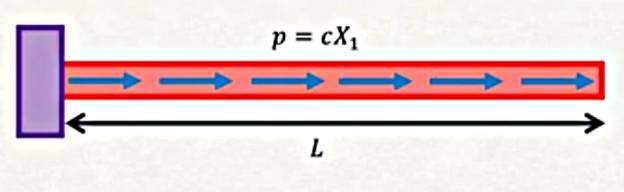
\includegraphics[width=20em]{compscieng_bpp45fem1_01.jpg}

Eksenel yükleme formülünü üstteki probleme uygulayınca

$$
EA \left( \frac{\ud^2 u}{\ud X_1^2}  \right) = -c X_1
$$

Eşitliğin sağındakileri sola geçirip her şeyi $EA$ ile bölersem, artık
(residual) hatasını bulabilirim,

$$
R =  \frac{\ud^2 u_{approx}}{\ud X_1^2} + \frac{c X_1}{EA}
$$







[devam edecek]

Kaynaklar

[1] Petitt, {\em Intro to the Finite Element Method}, University of Alberta,
    \url{https://www.youtube.com/watch?v=2iUnfPRk6Ro&list=PLLSzlda_AXa3yQEJAb5JcmsVDy9i9K_fi}

[2] Bayramlı, {\em Fizik, Materyel Mekanigi - 2}
    
[3] Bayramlı, {\em Fizik, Materyel Mekanigi - 4}
    
\end{document}





